% !TeX root = ../main.tex

% Design
% Explain the system design in detail
% Explain each system component sufficient details
% Explain workflows using algorithms
\chapter{Design}\label{chapter:design}
The following chapter presents the core design decisions that were taken to extend the Focaccia verifier with the reproducer.
Extra attention is given to the reproducer interface, the data taken from the verifier, and how it relates to the whole reproducer.
After a brief look at the interface, we will explore the reproducer and discuss in more detail how we create the environment for the reproduced program.
This step will go over the instructions we are trying to reproduce, along with setting up the registers, memory, and stack.

\section{Focaccia Interface}
The reproducer, which was designed as an add-on, comes after the verification process is done.
The verification process's output is a long list of calculations that occur at every step of the program's execution.

The result of these calculations is the following:
\begin{itemize}
    \item pc: The program counter can be used as a pseudo key that maps the calculations to the instruction or the basic block it belongs to. However, it is not a unique key since the same block can be repeated multiple times.
    \item txl: This is the difference between the current snapshot and the next one. This difference only includes registers.
    \item ref: These are the reference changes that happen during the execution of the instruction or the basic block. They are in the form of symbolic expressions and play a vital role when creating the reproducer program.
    \item errors: This is a list of errors found while comparing the emulator log with the symbolic execution. There are multiple levels of errors depending on their severity.
    \item snap: The snapshots are the concrete values that have been extracted. These include both register values and memory values.
\end{itemize}

Of the five entries mentioned, only two are essential for the reproducer, and an additional one is useful but not mandatory.
Another entry is used to identify bugs, whereas the final entry is not used at all.

\paragraph{errors:}
The verification process generates five different types of outputs, with errors being one of the key outputs.
They are used to filter through the output list to find exactly which steps have problems in them.
They are not necessarily used in the reproducer, but rather, they are used to pinpoint the places where the reproducer should be used.

\paragraph{txl:}
The next output, txl, does not directly contribute to the reproducer.
Since this output only shows the differences between the current and the next snapshot, it does not give any hints about the instructions.
Neither does it help find values that belong to the previous state of the execution process.
Therefore these values are not used in the reproducer.

\paragraph{pc:}
This entry is the program counter, and it is used to check whether the symbolic expression aligns with the snapshot.
We can use it this way since it is supposed to have the same value as the RIP register in x86.
Previously, we used it to find the location of the basic block that was turned into a symbolic expression.
However, updates to the verifier have made this step redundant since we can now directly convert symbolic expressions back into assembly instructions.

\paragraph{snap:}
The snapshot is one of the three inputs that the reproducer takes.
They are called snapshots because they represent the exact state of the CPU just before the instruction is executed.
However, snapshots contain far too much redundant information.
Most of these register and memory values are not used when executing our instruction/basic block.
We need a way to filter them in order to extract only the necessary values used in our setup.
This filtering step can be done by using symbolic expressions. 

\paragraph{ref:}
The final output is the ref, a symbolic expression representing the changes our snapshots undergo when we execute the next instruction.
These symbolic expressions have multiple purposes.
Firstly, they can be used to extract the assembly instructions needed for our program.
As mentioned before, we used to use the PC to extract the basic block, but with updates to the verifier, it became able to pinpoint the problematic instructions instead of the whole basic block.
This meant that extracting the instructions used would be difficult without getting the proper cutoff point.
Instead of trying to guess the actual point, the symbolic expression is used to get the exact instructions.

Secondly, the symbolic expression can be filtered to identify which registers are used for which cases.
These registers can be later matched with the correct values using the snapshots.
However, there is a special case of registers where this is more complex.
If the registers are used to address something in the memory, then we cannot simply copy the original value since these addresses would be wrong.
However, since the symbolic expressions can show exactly which memory values are changed, we can try to match them and handle them accordingly.

\section{Design of the Reproducer}
In this section, we will go over the design of the reproducer.
Since we have already explained the outputs of the verifier and how they relate to the reproducer, we will mainly concentrate on the different parts of the verifier.
The inner workings of the reproducer are depicted in figure \ref{fig:reproducer} in order to provide a clear picture of the data flow.
The creation process of the data section is shown in figure \ref{fig:data} while figure \ref{fig:text} shows the text section.

\begin{figure}[ht]
    \centering
    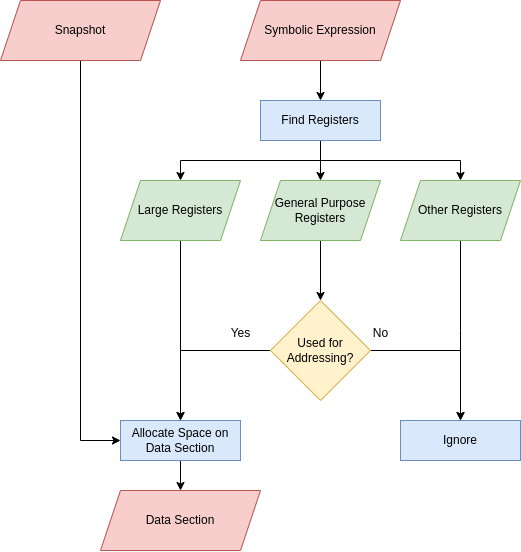
\includegraphics[width=0.8\linewidth]{figures/data}
    \caption{Process of creating the data section.}
    \label{fig:data}
\end{figure}

\begin{figure}[ht]
    \centering
    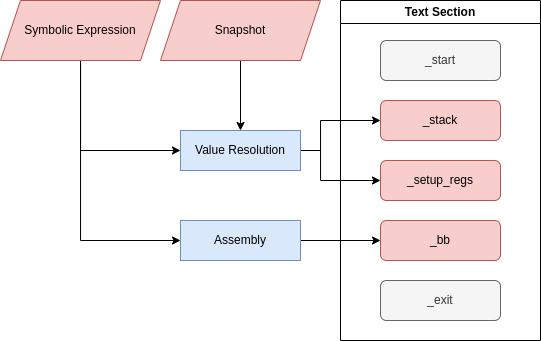
\includegraphics[width=0.8\linewidth]{figures/text}
    \caption{Process of creating the text section.}
    \label{fig:text}
\end{figure}

\subsection{Instructions and Basic Blocks}
The verifier was designed to reproduce bugs that come up in bigger programs.
This meant it needed to find the exact instruction that triggered it and run it without changing anything.
In our case, as depicted in the figure \ref{fig:text} this instruction is supplied by the symbolic expression and directly appended to the text section.
No adjustment is needed, so we append it without any change.

However, there is a slight problem in handling instructions that way.
This way of reproducing the bugs only lets us handle calculations.
If we tried the same thing with other instructions that changed the program flow, we would jump to unknown places with unknown consequences.
The same goes for instructions that affect hardware.
These special cases are handled in the following section.

\subsection{Registers}
Setting up registers according to their original values is also a very important part of the reproducer.
Some bugs might only be triggered when the registers are filled with special values.
To set the correct environment, we have to handle these values correctly.
Registers are used for two main purposes.
Firstly, they are used for general calculation.
In this case, we do not need to put too much thought into restoring these values.
However, in the second case, namely for addressing memory, we must be careful about which values we use.
The original values are most definitely wrong, as they are yet to be allocated.
Instead, we need to calculate different addresses where we know we can read from and write to.
Handling these registers is done in both the data and text sections.
Figure \ref{fig:data} shows where they are used in the data section, and figure \ref{fig:text} depicts the register setup in the code section.

The values of registers can be split into three categories as shown in figure \ref{fig:data}.
These categories are:
\begin{itemize}
    \item Large register values
    \item Address
    \item Other register values
\end{itemize}
All of these categories have different calculation methods, with some being rather straightforward and others needing multiple calculations where we leverage symbolic values for resolution.
In the following paragraphs, we will go into more detail about how they are calculated.

\paragraph{Large register values:}
Large registers are the common names we have given registers that cannot be filled directly with immediate values.
In these cases, even though we can easily extract the value from the snapshot, we cannot put them into assembly instructions.
Instead, we have to save the actual value in the memory as a constant and then use a special move instruction with the constant value's address to move it to the register.

We handle these in two steps.
In the first step, we save these register values to the data section.
Then, when we write the values into the registers, we use the aforementioned special move instructions with the addresses.
This way, we can simply set these large registers.

\paragraph{Addreses:}
These values are generally inside the 64-bit general-purpose registers.
The assembly instructions use them for read or write operations.
Unlike the other types of instructions, we cannot simply copy them because they point to memory locations that only exist for the original program.
Instead, we need to allocate space in the data section and then change every address pointing to the original one with the new one.

When doing this, we need to take care of a couple of details.
Firstly, we can both read and write in the same memory location.
In this case, we need to be aware that this address is used in multiple places and not create a new one.

The second case concerns the readable and writeable chunk sizes and how they align.
We might need to read and write to a continuous memory chunk.
However, the data from the symbolic expression might point to a random order of reads and writes that don't even align with the size.
In this case, we might order these addresses, but the size of the reads and writes might cause confusion.
To prevent problems from arising, we split all of these memory locations into bytes.
This means we always have an address for any byte that is read or written to.
In figure \ref{fig:addr_match}, we can see a comparison of the naive approach and our approach.

\begin{figure}[ht]
    \centering
    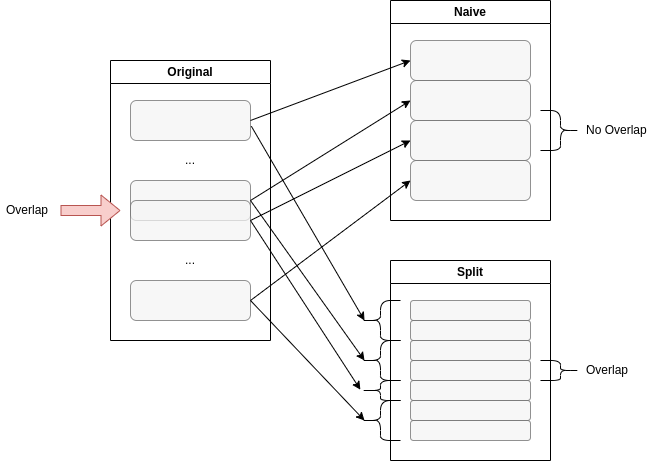
\includegraphics[width=0.8\linewidth]{figures/alloc2}
    \caption{Naive approach to data allocation versus our strategy.}
    \label{fig:addr_match}
\end{figure}

\paragraph{Other register values for calculation:}
Finally, we have all of the other registers.
These registers can be set by immediate values.
This makes setting them up rather easy since we just need to read the values from the snapshot and use the correct move instruction according to their type. 

\subsection{Memory}
In the last subsection, we have an overview about using addresses but the actual method of finding these addresses is a bit more complicated.
We can gather three subsets of symbolic information from the one we have been given. These are:
\begin{itemize}
    \item Used memory addresses
    \item Changed memory addresses
    \item Used registers
\end{itemize}

By using the first two items, we can find which values are used to address memory.
However, these would be just the addresses and not the actual values of the registers.
In x86, an address can be made out of base, index, scale, and displacement.
Out of these four parts, the first two are registers, and the latter are constants.
Only the base is necessary, while the other ones can be omitted.
This means there are multiple ways an address's symbolic expression can look.

In order to solve this address evaluation, we use a shortcut.
We can separate the offset from the base by evaluating the base register and the whole address.
When we prepare the new address, we can subtract this offset from the displacement.
This will allow us to allocate space in the data section and ignore the offset when running the code.
This calculation is depicted in figure \ref{fig:mem_addr}.
Using this method, we can keep the original values for everything except the base and don't need to consider how the addressing is made.

\begin{figure}[ht]
    \centering
    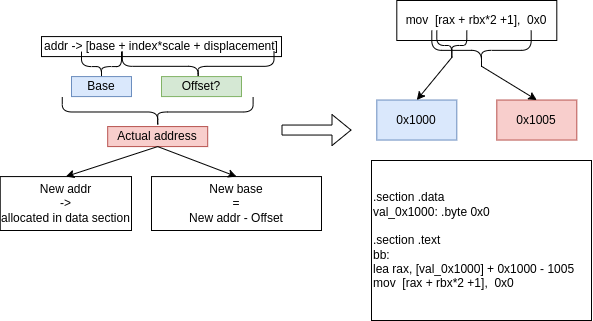
\includegraphics[width=0.9\linewidth]{figures/mem_addr}
    \caption{Calculating the offset to match the allocated address.}
    \label{fig:mem_addr}
\end{figure}

\subsection{Stack}
Setting the stack state is the final step in configuring the reproducer.
This step isn't required for every instruction but is essential for operations that involve the stack, such as push, pop, or any memory addressing that relies on the stack pointer.
The method for finding the values in the stack is the same as the memory values; we evaluate expressions related to memory reads or writes.
However, we pay special attention to whether these symbolic expressions involve the stack pointer.

Although the approach for identifying stack values mirrors that used for general memory operations, initializing these stack values demands a different method.
Unlike other memory operations where the exact location is flexible as long as there's enough space and the registers have the correct addresses, the values in the stack need to be in the correct positions.
Therefore, the values related to the original stack must maintain their relative positions relative to the stack pointer.

We first need to gather the correct values to reconstruct the stack.
Generally, not all of the values on the stack are used for the instructions given.
Therefore, we cannot recognize them.
In that case, we substitute these values with zeros.
When collecting these values and adding the padding, it is essential to remember that the values are not only before (in higher addresses) the stack pointer but also after (in lower addresses) it.
This means we need to put all the values into the stack and then ensure the stack pointer is in the correct place.
We do this by pushing all the values to the stack and subtracting the number of bytes whose addresses are smaller than the original stack pointer from the new stack pointer.
By using this method, we recreated the stack.

\begin{figure}[ht]
    \centering
    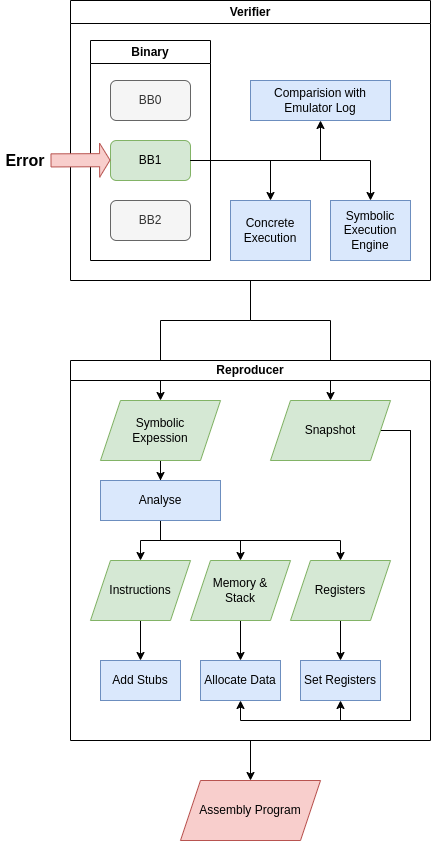
\includegraphics[width=0.6\linewidth]{figures/rep}
    \caption{Overview of the Reproducer.}
    \label{fig:reproducer}
\end{figure}
